\begin{figure}[t]
    \centering
    \begin{subfigure}[b]{.24\linewidth}
        \centering
        \resizebox{\linewidth}{!}{\includegraphics{figure/plot/reference/fig9b-covert-vm-summary.pdf}}
        \caption{\label{fig:9b:ref:covert-vm-summary}[Ref]Channel performance.}
    \end{subfigure}
    \hfill
    \begin{subfigure}[b]{.24\linewidth}
        \centering
        \resizebox{\linewidth}{!}{\includegraphics{figure/plot/reference/fig9c-covert-vm-signal-receiver.tikz.pdf}}
        \caption{\label{fig:9c:ref:covert-vm-signal}[Ref]Channel receiver signal.}
    \end{subfigure}
    \hfill
    \begin{subfigure}[b]{.24\linewidth}
        \centering
        \resizebox{\linewidth}{!}{\includegraphics{example-image-duck}}
        % \resizebox{\linewidth}{!}{\includegraphics{figure/plot/reproduce/fig9b-covert-vm-summary.pdf}}
        \caption{\label{fig:9b:rep:covert-vm-summary}[Rep]Channel performance.}
    \end{subfigure}
    \hfill
    \begin{subfigure}[b]{.24\linewidth}
        \centering
        \resizebox{\linewidth}{!}{\includegraphics{example-image-duck}}
        % \resizebox{\linewidth}{!}{\includegraphics{figure/plot/reproduce/fig9c-covert-vm-signal-receiver.tikz.pdf}}
        \caption{\label{fig:9c:rep:covert-vm-signal}[Rep]Channel receiver signal.}
    \end{subfigure}

    \caption{\label{fig:5:cross-vm-covert}Cross-VM covert channel.}
\end{figure}
